\section{Graph Contraction}\\

    \noindent Graph contraction itself is trivial, but what is needed is a method of contracting the graph while retaining all information about
    the original graph to enable routing points to be re-inserted.

    \vspace{12pt}\subsection{Initial Contraction}
    \noindent The following figure illustrates a non-contracted graph. Consider a process of contraction which starts by removal of the vertex B.

    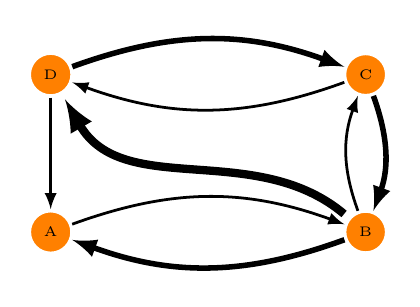
\begin{tikzpicture}[font=\tiny]
    \tikzstyle{node_style} = [draw=white, very thick, circle, fill=orange]
    \tikzstyle{arrow_style1} = [->, black, line width=1, >=latex]
    \tikzstyle{arrow_style2} = [->, black, line width=2, >=latex]
    \tikzstyle{arrow_style3} = [->, black, line width=3, >=latex]
    \tikzstyle{edge_style2} = [lightgray, line width=1]


    \node[node_style] (n1) at (0,0) {A};
    \node[node_style] (n2) at (4,0) {B};
    \node[node_style] (n3) at (4,2) {C};
    \node[node_style] (n4) at (0,2) {D};

    \draw[arrow_style1] (n1) edge [bend left=20] (n2);
    \draw[arrow_style2] (n2) edge [bend left=20] (n1);
    \draw[arrow_style1] (n2) edge [bend left=20] (n3);
    \draw[arrow_style2] (n3) edge [bend left=20] (n2);
    \draw[arrow_style1] (n3) edge [bend left=20] (n4);
    \draw[arrow_style2] (n4) edge [bend left=20] (n3);
    \draw[arrow_style1] (n4) edge (n1);
    \draw[arrow_style3, shorten <=2pt, shorten >=2pt] (n2) edge [out=140, in=-60] (n4);
\end{tikzpicture}


    \noindent Contraction requires a `vert2edge` map, and a list in each edge of mappings on to original edges in the full graph. The former of
    these is an unsorted set, initiated as,
    \begin{lstlisting}
        vert2edge(A) = [2, 5]
        vert2edge(B) = [2, 5, 3, 6]
        vert2edge(C) = [3, 6, 7, 4]
        vert2edge(D) = [7, 4]
    \end{lstlisting}
    Consider the removal of vertex {\tt B}, with new edges {\tt(2, 3) -> 8} and {\tt(6, 5) -> 9}. These new edges then hold
    \begin{lstlisting}
        edge(8).old = [2, 3]
        edge(9).old = [6, 5]
    \end{lstlisting}
    And the `vert2edge` maps for {\tt A}, {\tt B}, and {\tt C} need to be updated to,
    \begin{lstlisting}
        vert2edge(A) = [8, 9]
        vert2edge(B) = [8, 9]
        vert2edge(C) = [8, 9, 7, 4]
    \end{lstlisting}
    where {\tt vert2edge(B)} is retained in updated form to allow subsequent re-insertion.  This reduces the graph to:
    \pagebreak

    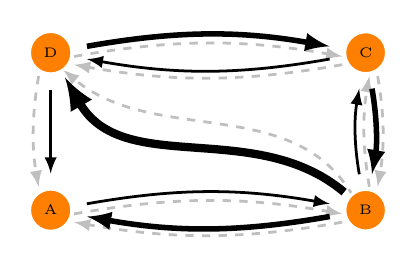
\begin{tikzpicture}[font=\tiny, >=latex, shorten >=5pt, shorten <=5pt]
    \tikzstyle{nonode} = []
    \tikzstyle{node_style} = [draw=white, very thick, circle, fill=orange]
    \tikzstyle{black_arrow1} = [->, black, line width=1]
    \tikzstyle{black_arrow2} = [->, black, line width=2]
    \tikzstyle{black_arrow3} = [->, black, line width=3]
    \tikzstyle{grey_arrow} = [->, lightgray, dashed, line width=1]

    \node[nonode] (nAd) at (0,-0.1) {};
    \node[nonode] (nAl) at (-0.1,0) {};
    \node[nonode] (nBd) at (4,-0.1) {};
    \node[nonode] (nBr) at (4.1,0) {};
    \node[nonode] (nCd) at (4,1.9) {};
    \node[nonode] (nCr) at (4.1,2) {};
    \node[nonode] (nDd) at (0,1.9) {};
    \node[nonode] (nDl) at (-0.1,2) {};

    \draw[grey_arrow] (nAd) edge [bend left=10] (nBd);
    \draw[grey_arrow] (nBd) edge [bend left=10] (nAd);
    \draw[grey_arrow] (nBr) edge [bend left=10] (nCr);
    \draw[grey_arrow] (nCr) edge [bend left=10] (nBr);
    \draw[grey_arrow] (nCd) edge [bend left=10] (nDd);
    \draw[grey_arrow] (nDd) edge [bend left=10] (nCd);
    \draw[grey_arrow] (nDl) edge [bend right=10] (nAl);
    \draw[grey_arrow] (nBd) edge [out=120, in=-40] (nDl);

    \node[node_style] (nA) at (0,0) {A};
    \node[node_style] (nB) at (4,0) {B};
    \node[node_style] (nC) at (4,2) {C};
    \node[node_style] (nD) at (0,2) {D};

    \draw[black_arrow1] (nA) edge [bend left=10] (nB);
    \draw[black_arrow2] (nB) edge [bend left=10] (nA);
    \draw[black_arrow1] (nB) edge [bend left=10] (nC);
    \draw[black_arrow2] (nC) edge [bend left=10] (nB);
    \draw[black_arrow1] (nC) edge [bend left=10] (nD);
    \draw[black_arrow2] (nD) edge [bend left=10] (nC);
    \draw[black_arrow1] (nD) edge (nA);

    \draw[black_arrow3, shorten <=2pt, shorten >=2pt] (nB) edge [out=140, in=-60] (nD);
\end{tikzpicture}


    The {\tt edge(.).old} sets are *ordered* and so must be constructed with the following pseudo-code:
    \begin{lstlisting}
        vert2rm = B
        # replace vertex:
        nbs = vert2rm.get_all_neighbours()
        vtx0 = vertex_map (nbs [0]) # = vertex A
        vtx1 = vertex_map (nbs [1]) # = vertex B
        vtx0.replace_neighbour (vert2rm, nbs [1])
        vtx1.replace_neighbour (vert2rm, nbs [0])

        edges2rm = vert2edge(b) = [2, 5, 3, 6]
        newe = 8
        if (vert2rm.is_double)
            newe = c (newe, newe++) # [8, 9]
        for ne in newedgenum:
            # insert in edge first
            for e in edges2rm:
                if e.from == nbs [0]:
                    if edge(e).old.size () > 0:
                        edge(newe).old = edge(e).old
                    else
                        edge(newe).old = e
                    edges2rm.erase (e)
                    vert2edge(vert2rm).erase (e)
                    stop
            # ne = 8: e = 2; edge2rm = [5, 3, 6]; edges(8).old = 2
            # ne = 9: e = 6; edge2rm = [5]; edges(9).old = 6

            # then out edge:
            for e in edges2rm:
                if e in vert2rm.out:
                    if edge(e).old.size() > 0:
                        edge(newe).old = c (edge(newe).old, edge(e).old)
                    else:
                        edge(newe).old = c (edge(newe).old, e)
                    edges2rm.erase (e)
                    vert2edge(vert2rm).erase (e)
                    stop
            # ne = 8: e = 3; edge2rm = [5, 6]; edges(8).old = [2, 3]
            # ne = 9: e = 5; edge2rm = []; edges(9).old = [6, 5]
            # update vert2edge map:
            vert2edge(vert2rm).insert(ne)
    \end{lstlisting}
    So replacing vertex {\tt B} gives the following maps:
    \begin{lstlisting}
        vert2edge(A) = [8, 9]
        vert2edge(B) = [8, 9]
        vert2edge(C) = [8, 9, 7, 4]
        vert2edge(D) = [7, 4]
        edge(8).old  = [2, 3]
        edge(9).old  = [6, 5]
    \end{lstlisting}
    Then consider removal of vertex {\tt C} according to the same pseudo-code, with {\tt vert2rm = C}, {\tt vtx0 = A}, {\tt vtx1 = D}, and {\tt
    newedgenum = [10, 11]}. The code then iterates through the following values:
    \begin{lstlisting}
        ne = 10
        # in-edge:
        e = 8
        edge(e).old = [2, 3]
        edge(10).old = edge(8).old = [2, 3]
        # out-edge:
        e = 4
        edge(10).old = c(edge(10).old, 4) = [2, 3, 4]

        ne = 11
        # in-edge:
        e = 7
        edge(11).old = 7
        # out-edge:
        e = 9
        edge(11).old = c(edge(11).old, edge(e).old) = [7, 6, 5]
    \end{lstlisting}
    This finally gives the desired contraction with the following mappings:
    \begin{lstlisting}
        vert2edge(A, B, C, D) = [10, 11] # all the same
        edge(10).old = [2, 3, 4]
        edge(11).old = [7, 6, 5]
    \end{lstlisting}


    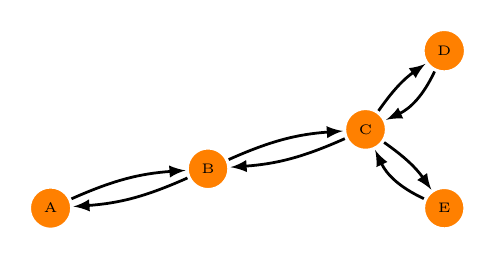
\begin{tikzpicture}[font=\tiny]
    \tikzstyle{node_style} = [draw=white, very thick, circle, fill=orange]
    \tikzstyle{arrow_style1} = [->, black, line width=1, >=latex]

    \node[node_style] (n1) at (0,0) {A};
    \node[node_style] (n2) at (2,0.5) {B};
    \node[node_style] (n3) at (4,1) {C};
    \node[node_style] (n4) at (5,2) {D};
    \node[node_style] (n5) at (5,0) {E};

    \draw[arrow_style1] (n1) edge [bend left=10] (n2);
    \draw[arrow_style1] (n2) edge [bend left=10] (n1);
    \draw[arrow_style1] (n2) edge [bend left=10] (n3);
    \draw[arrow_style1] (n3) edge [bend left=10] (n2);
    \draw[arrow_style1] (n3) edge [bend left=10] (n4);
    \draw[arrow_style1] (n4) edge [bend left=20] (n3);
    \draw[arrow_style1] (n3) edge [bend left=10] (n5);
    \draw[arrow_style1] (n5) edge [bend left=20] (n3);
    %\draw[arrow_style3, shorten <=2pt, shorten >=2pt] (n2) edge [out=140, in=-60] (n4);
\end{tikzpicture}


    \vspace{12pt}\subsection{Graph reconstruction}

    \noindent The maps can then be used to reconstruct a graph. Consider the re-insertion of Vertex {\tt B} to give the graph of
    Fig.~\ref{fig:4}.
    
    \begin{figure}[ht!]
    \psset{unit=8mm}
    \begin{center}
        \psset{griddots=0,gridlabels=7pt,subgriddiv=1}
        \newgray{lightgrey}{0.75}
        \begin{pspicture} (0,-0.5) (18,6)
            \cnodeput[fillstyle=solid,fillcolor=orange,linecolor=gray,linewidth=2pt] (0,3){A}{A}
            \cnodeput[fillstyle=solid,fillcolor=orange,linecolor=gray,linewidth=2pt] (6,3){B}{B}
            \cnodeput[fillstyle=solid,fillcolor=orange,linecolor=gray,linewidth=2pt] (12,3){C}{C}
            \cnodeput[fillstyle=solid,fillcolor=orange,linecolor=gray,linewidth=2pt] (18,3){D}{D}

            \rput(3,4){\rnode{n2}{2}}
            \rput(9,4){\rnode{n3}{3}}
            \rput(15,4){\rnode{n4}{4}}
            \rput(3,5){\rnode{n12}{12}}
            \rput(12,5){\rnode{n13}{13}}
            \rput(9,6){\rnode{n10}{10}}

            \rput(3,2){\rnode{n5}{5}}
            \rput(9,2){\rnode{n6}{6}}
            \rput(15,2){\rnode{n7}{7}}
            \rput(3,1){\rnode{n15}{15}}
            \rput(12,1){\rnode{n14}{14}}
            \rput(9,0){\rnode{n11}{11}}

            \nccurve[linewidth=2pt,nodesep=5pt,angleA=40,angleB=180,arrowsize=1.5pt 4]{->}{A}{n12}
            \nccurve[linewidth=2pt,nodesep=5pt,angleA=0,angleB=140,arrowsize=1.5pt 4]{->}{n12}{B}
            \nccurve[linewidth=2pt,nodesep=5pt,angleA=60,angleB=180,arrowsize=1.5pt 4]{->}{B}{n13}
            \nccurve[linewidth=2pt,nodesep=5pt,angleA=0,angleB=120,arrowsize=1.5pt 4]{->}{n13}{D}

            \nccurve[linewidth=0.5pt,linestyle=dashed,nodesep=5pt,linecolor=lightgrey,angleA=40,angleB=180,arrowsize=1.5pt 8]{->}{A}{n2}
            \nccurve[linewidth=0.5pt,linestyle=dashed,nodesep=5pt,linecolor=lightgrey,angleA=0,angleB=140,arrowsize=1.5pt 8]{->}{n2}{B}
            \nccurve[linewidth=0.5pt,linestyle=dashed,nodesep=5pt,linecolor=lightgrey,angleA=40,angleB=180,arrowsize=1.5pt 8]{->}{B}{n3}
            \nccurve[linewidth=0.5pt,linestyle=dashed,nodesep=5pt,linecolor=lightgrey,angleA=0,angleB=140,arrowsize=1.5pt 8]{->}{n3}{C}
            \nccurve[linewidth=0.5pt,linestyle=dashed,nodesep=5pt,linecolor=lightgrey,angleA=40,angleB=180,arrowsize=1.5pt 8]{->}{C}{n4}
            \nccurve[linewidth=0.5pt,linestyle=dashed,nodesep=5pt,linecolor=lightgrey,angleA=0,angleB=140,arrowsize=1.5pt 8]{->}{n4}{D}

            \nccurve[linewidth=2pt,nodesep=5pt,angleA=-40,angleB=180,arrowsize=1.5pt 4]{<-}{A}{n15}
            \nccurve[linewidth=2pt,nodesep=5pt,angleA=0,angleB=220,arrowsize=1.5pt 4]{<-}{n15}{B}
            \nccurve[linewidth=2pt,nodesep=5pt,angleA=-60,angleB=180,arrowsize=1.5pt 4]{<-}{B}{n14}
            \nccurve[linewidth=2pt,nodesep=5pt,angleA=0,angleB=240,arrowsize=1.5pt 4]{<-}{n14}{D}

            \nccurve[linewidth=0.5pt,linestyle=dashed,nodesep=5pt,linecolor=lightgrey,angleA=-40,angleB=180,arrowsize=1.5pt 8]{<-}{A}{n5}
            \nccurve[linewidth=0.5pt,linestyle=dashed,nodesep=5pt,linecolor=lightgrey,angleA=0,angleB=220,arrowsize=1.5pt 8]{<-}{n5}{B}
            \nccurve[linewidth=0.5pt,linestyle=dashed,nodesep=5pt,linecolor=lightgrey,angleA=-40,angleB=180,arrowsize=1.5pt 8]{<-}{B}{n6}
            \nccurve[linewidth=0.5pt,linestyle=dashed,nodesep=5pt,linecolor=lightgrey,angleA=0,angleB=220,arrowsize=1.5pt 8]{<-}{n6}{C}
            \nccurve[linewidth=0.5pt,linestyle=dashed,nodesep=5pt,linecolor=lightgrey,angleA=-40,angleB=180,arrowsize=1.5pt 8]{<-}{C}{n7}
            \nccurve[linewidth=0.5pt,linestyle=dashed,nodesep=5pt,linecolor=lightgrey,angleA=0,angleB=220,arrowsize=1.5pt 8]{<-}{n7}{D}

            \nccurve[linewidth=1pt,linestyle=dashed,linecolor=lightgrey,nodesep=5pt,angleA=60,angleB=180,arrowsize=1.5pt 4]{->}{A}{n10}
            \nccurve[linewidth=1pt,linestyle=dashed,linecolor=lightgrey,nodesep=5pt,angleA=0,angleB=120,arrowsize=1.5pt 4]{->}{n10}{D}

            \nccurve[linewidth=1pt,linestyle=dashed,linecolor=lightgrey,nodesep=5pt,angleA=-60,angleB=180,arrowsize=1.5pt 4]{<-}{A}{n11}
            \nccurve[linewidth=1pt,linestyle=dashed,linecolor=lightgrey,nodesep=5pt,angleA=0,angleB=240,arrowsize=1.5pt 4]{<-}{n11}{D}
        \end{pspicture}
    \end{center}

    \captionsetup{format=hang}
    \caption{Network of Fig.~\ref{fig:1} contracted through removal of vertices B \& C.}
\label{fig:4}
\end{figure}


    Vertex B only exists in the {\tt vert2edge} map as,
    \begin{lstlisting}
        vert2edge(B) = [10, 11]
    \end{lstlisting}
    Then trace both of those edges, extracting the relevant info from the original graph:
    \begin{lstlisting}
        olde = 10
        newe = 12
        v2insert = B
        e = edge(olde).old = [2, 3, 4]
        vlist = e[1].from # = A
        vert2edge(vlist[1]).erase(olde)
        vert2edge(vlist[1]).insert(newe)
        elist = []
        d = w = 0
        for i in e:
            vlist.push_back(e.to)
            vert2edge(e.to).erase(olde)
            vert2edge(e.to).insert(newe)
            elist.push_back(e)
            d += graph(e).d
            w += graph(e).w
            if (e.to == v2insert)
                vlist1 = vlist
                elist1 = elist
                vlist = e.to
                d1 = d
                w1 = w
                d = w = 0
                edge(newe).old = elist
                elist = []
                newe++
                vert2edge(v2inert).insert(newe)
        edge(newe).old = elist
        edge(olde).erase
    \end{lstlisting}
    A first pass for edge\#10 will give the following values
    \begin{lstlisting}
        newe = 12
        vert2edge(A) = [10, 11] -> [12, 11]
        vlist = [A]
        e = edge(10).old = [2, 3, 4]
        (for i in e:)

        # e = 2
        vlist = [A, B]
        vert2edge(B) = [10, 11] -> [12, 11]
        elist = 2
        edge(12).old = 2
        vlist1 = vlist # = [A, B]
        elist1 = elist # = 2
        vlist = [B]
        elist = []
        newe = 13
        vert2edge(B) = [12, 11, 13]

        # e = 3
        vlist = [B, C]
        vert2edge(C) = [10, 11] -> [13, 11]
        elist = 3

        # e = 4
        vlist = [B, C, D]
        vert2edge(D) = [10, 11] -> [13, 11]
        elist = [3, 4]

        # out of loop so
        edge(13).old = [3, 4]
    \end{lstlisting}
    This gives the following:
    \begin{lstlisting}
        vert2edge(A) = [12, 11]
        vert2edge(B) = [12, 11, 13]
        vert2edge(C, D) = [13, 11]
        edge(12).old = [2]
        edge(13).old = [3, 4]
    \end{lstlisting}
    Subsequently tracing the second edge\#11 with {\tt edge(11).old = [7, 6, 5]} gives,
    \begin{lstlisting}
        newe = 14
        vert2edge(D) = [13, 11] -> [13, 14]
        e = [7, 6, 5]
        vlist = [D]
        (for i in e:)

        # e = 7
        vlist = [D, C]
        vert2edge(C) = [13, 11] -> [13, 14]
        elist = 7

        # e = 6
        vlist = [D, C, B]
        elist = [7, 6]
        vert2edge(B) = [12, 11, 13] -> [12, 13, 14]
        edge(14).old = [7, 6]
        vlist1 = vlist # = [D, C, B]
        elist1 = elist # = [7, 6]
        vlist = [B]
        elist = []
        newe = 15
        vert2edge(B) = [12, 13, 14, 15]

        # e = 5
        vlist = [B, A]
        elist = 5
        vert2edge(A) = [12, 11] -> [12, 15]

        # out of loop so
        edge(15).old = [5]
    \end{lstlisting}
    This gives the following final mappings:
    \begin{lstlisting}
        vert2edge(A)    = [12, 15]
        vert2edge(B)    = [12, 13, 14, 15]
        vert2edge(C, D) = [13, 14]
        edge(12).old = [2]
        edge(13).old = [3, 4]
        edge(14).old = [7, 6]
        edge(15).old = [5]
    \end{lstlisting}
    And that's it!

